\documentclass[10pt,twocolumn,letterpaper]{article}
\usepackage[english]{babel}
\usepackage{blindtext}
\usepackage{cvpr}
\usepackage{times}
\usepackage{epsfig}
\usepackage{graphicx}
\graphicspath{{images/}}
\usepackage{amsmath}
\usepackage{amssymb}
\usepackage{caption}
\usepackage[breaklinks=true,bookmarks=false]{hyperref}

\cvprfinalcopy

\def\httilde{\mbox{\tt\raisebox{-.5ex}{\symbol{126}}}}

\title{\LARGE FormulaTour}

\author{Gianluca Capozzi\\
	"La Sapienza" University of Rome\\
	{\tt\small capozzi.1693255@studenti.uniroma1.it}
	\and
	Marco Costa\\
	"La Sapienza" University of Rome\\
	{\tt\small costa.1691388@studenti.uniroma1.it}
}


\begin{document}
\twocolumn[{%
	\renewcommand\twocolumn[1][]{#1}%
	\maketitle
	\begin{center}
		\centering
		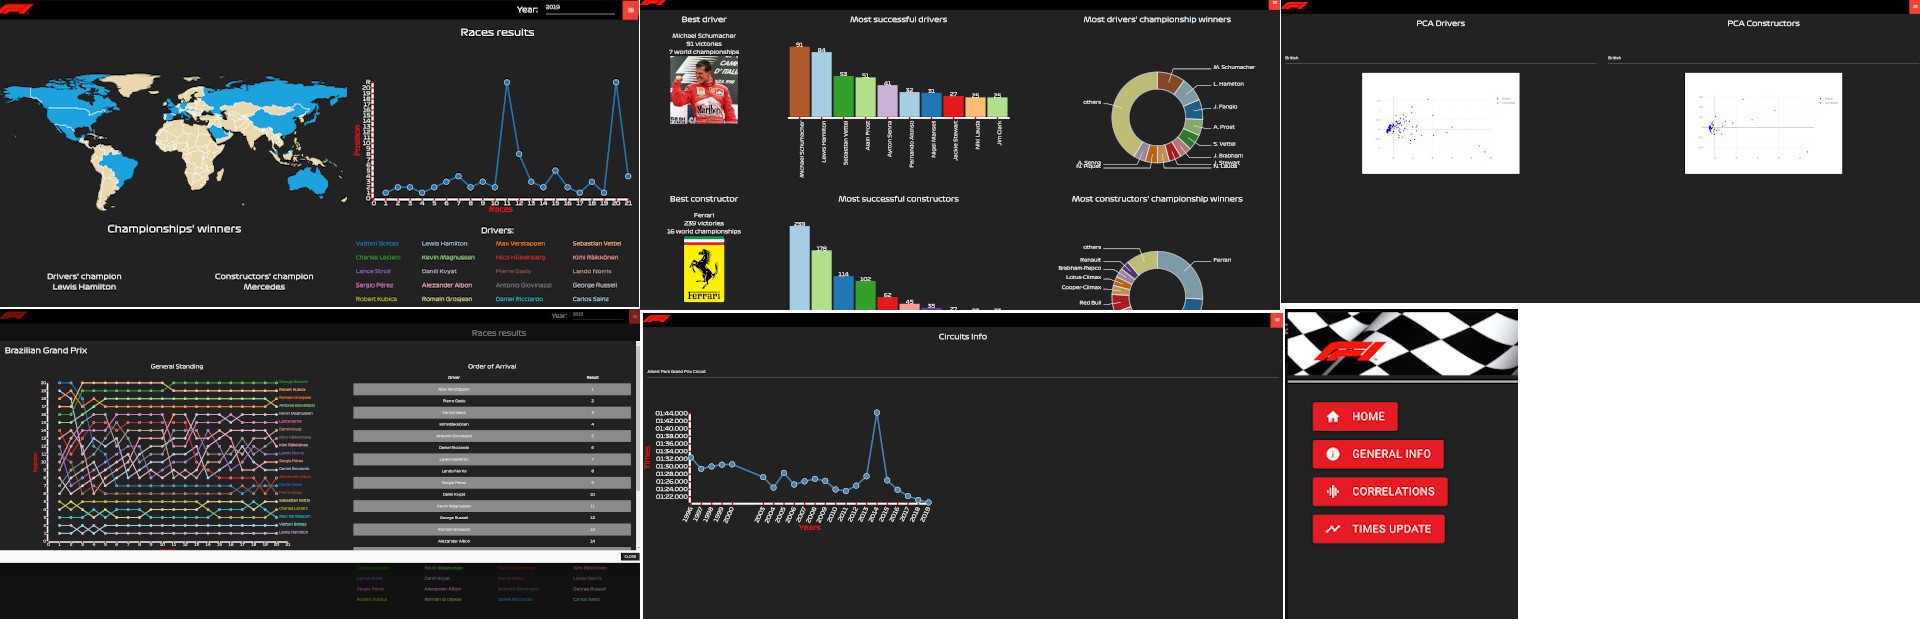
\includegraphics[width=\textwidth]{allViews}
		\captionof{figure}{Framework Views}
	\end{center}%
}]

\begin{abstract}
   \blindtext
\end{abstract}

\section{Introduction}
Introduction text 
\blinddocument

\section{Dataset}


\section{Visualization}


\section{Analytics}


\section{Conclusion}
Conclusion text

\end{document}
